\chapter{Efficient algebraic computation algorithms}\label{chap:algebraic}
%\todo[inline,size=\small]{este capitulo e basedado no livro Introduction to
%algorithms. retirei as partes com explicacoes mais detalhadas, para ficar so
%com uma visao mais geral.}

Almost all existing cryptographic primitives offering more than the most basic
of functionalities heavily relies on algebraic operations.
%Most of all the current cryptographic primitives rely heavily on algebraic
%operations.
That is why when implementing such primitives one must pay special attention to
the way these algebraic operations are performed. The ``classical'' textbook
way may be efficient enough for small (and not so practical) parameters, but
when dealing with thousand bit numbers things become noticeably slow.

In \citescheme{catalano:fiore:2013}'s homomorphic evaluation, more precisely
\GateEval is the critical and the slowest operation and thus needs to be
implemented as efficiently as possible. This sub-routine is simply an
arithmetic circuit evaluation, but instead of using input values from field
$\bbF_p$ , it uses polynomial coefficients from $\bbF_p[X]$ as a result of
previous \Auth's or \Eval's of $n$ messages. Sum gates and product gates
compute the addition and multiplication of two polynomials, respectively.

To the sum gate there isn't much that we can do since the straightforward
algorithm takes $\Theta(n)$. On the other hand, the product gate is where a big
optimization can be introduced. The straightforward method of multiplication
takes $\Theta(n^2)$, and for big enough values of $n$, this becomes extremely
slow, and therefore compromises the efficiency of the entire homomorphic
scheme. So it is obvious that this is where we have to find some more efficient
algorithms in order to reduce this time complexity. As for the multiply by
a constant, the straightforward way is $\Theta(n)$ as well.
Following on the suggestion by \citeauthor{catalano:fiore:2013}, the product
problem can be mitigated by using algorithms based on the fast Fourier
Transform (FFT), which can reduce the multiplication of two polynomials to
$\Theta(n \log n)$.

Fourier Transforms are widely used in signal processing, and without them we
wouldn't have much of the technological developments of today. A signal is
given in the \emph{time domain}: as a function mapping time to amplitude. The
Fourier analysis allows us to express the signal as a weighted sum of
phase-shifted sinusoids of varying frequencies. The weights and phases
associated with the frequencies characterize the signal in the \emph{frequency
domain}. Fast Fourier analysis is widely employed in many of our applications
of today: audio recording, MP3 audio compression or JPEG image encoding and
compression.

Signal processing is just one of the many applications of Fourier Transforms.
One other field where it can be used, and the one of interest to us, is where
it can be used to perform an efficient multiplication of two polynomials.

\section{Polynomials}
A \emph{polynomial} in the variable $x$ over the field $\bbF$ can be
represented as a summation like:
\begin{equation*}
  P(x) = \sum_{i = 0}^{n - 1}{p_i x^i}
\end{equation*}
The $p_i$ values are the \emph{coefficients} of the polynomial, and are drawn
from the underlying field $\bbF$. The degree of the polynomial $P(x)$ is $d$ if
its highest nonzero coefficient is $p_d$; we denote it by $\Degree(P) = d$. Any
integer strictly greater than the degree of the polynomial is the
\emph{degree-bound} of that polynomial. The degree of a polynomial of
degree-bound $n$ may be any integer between $0$ and $n - 1$, inclusive. The
usual operations over polynomials, and the ones that are of interest to us, are
addition and multiplication.

For polynomial addition, if $A(x)$ and $B(x)$ are polynomials of degree-bound
$n$:
\begin{equation*}
  A(x) = \sum_{i = 0}^{n - 1}{a_i x^i}
  \quad
  \text{and}
  \quad
  B(x) = \sum_{i = 0}^{n - 1}{b_i x^i},
\end{equation*}
their sum is a polynomial $C(x) = A(x) + B(x)$, also of degree-bound $n$, as:
\begin{equation}
  C(x) = \sum_{i = 0}^{n - 1}{c_i x^i},
  \quad \text{such that $c_i = a_i + b_i$}
  \label{eq:poly_sum1}
\end{equation}
As a result, it holds that $\Degree(C) = \max(\Degree(A), \Degree(B))$.

The straightforward way of multiplying two polynomials $A(x)$ and $B(x)$ of
degree-bound $n$, resulting in the product $C(x) = A(x) B(x)$ of degree bound
$2n - 1$, is expressed as:
\begin{equation}
  C(x) = \sum_{i = 0}^{2n-2}{c_i x^i},
  \quad \text{such that each $c_i = \sum_{j = 0}^{i}{a_j b_{i - j}}$}
  \label{eq:poly_mul1}
\end{equation}
If $A(x)$ and $B(x)$ are of degree-bound $n_a$ and $n_b$, respectively, and
since that clearly $\Degree(C) = \Degree(A) + \Degree(B)$, then $C(x)$ is of
degree-bound $n_a + n_b - 1$. Because every polynomial of degree-bound $n$ is
also of degree-bound $n + 1$, we can also say that $C(x)$ is of degree-bound
$n_a + n_b$.

\subsection{Representation}
The way we represent polynomials can be directly related to the time it takes
to execute some operation over them, especially in the case of multiplication.
We now present the two common representations, which are the ones used to
obtain a faster polynomial multiplication with FFT.

\paragraph*{Coefficient representation}
The most natural and simple representation is the \emph{coefficient
representation}, where a polynomial $A(x) = \sum_{i = 0}^{n - 1}{a_i x^i}$ of
degree-bound $n$ is represented as a vector of coefficients $a
= (\setSpace{a}{0}{n-1})$.

This representation is very convenient for some operations. For instance, the
evaluation of the polynomial $A(x)$ at a given point $x_0$ can be done in
$\Theta(n)$ time using \emph{Horner's rule}:
\begin{equation*}
  A(x_0) = a_0 + x_0 (a_1 + x_0(a_2 + \dotsc + x_0(a_{n - 2} + x_0(a_{n - 1}))
  \dotsc, ))
\end{equation*}

Adding two polynomials in coefficient representation is also very simple:
having two vectors $a$ and $b$ representing the polynomials $A(x)$ and $B(x)$,
respectively, the addition is simply their vector addition $c = (a_0 + b_0,
\dotsc, a_{n - 1} + b_{n - 1})$ which takes $\Theta(n)$ time.

But if we look at polynomial multiplication (with coefficient representation)
of two polynomials $A(x)$ and $B(x)$ of degree-bound $n$, we get
a multiplication with $\Theta(n^2)$ time. That is because we have to multiply
each coefficient of vector $a$ by each coefficient in vector $b$. The resulting
vector $c$ is also called the \emph{convolution} of the input vectors $a$ and
$b$, denoted as $c = a \otimes b$.

\paragraph*{Point-value representation}
A \emph{point-value representation} of a polynomial $A(x)$ of degree-bound $n$
is a set of \emph{$n$ point-value pairs}
\begin{equation*}
  \{ (x_0, y_0), \dotsc, (x_{n-1}, y_{n-1}) \}
\end{equation*}
such that all $x_i$ are \emph{distinct} and for each $i = 0, \dotsc, n-1$ it
holds that $y_i = A(x_i)$. A polynomial has many different point-value
representations since we can choose any set of $n$ distinct points
$\setSpace{x}{0}{n-1}$.

The conversion from coefficient to point-value representation is simple:
select $n$ distinct points
%Going from coefficient to point-value representation is straightforward in
%principle, since all we have to do is select $n$ distinct points
$\setSpace{x}{0}{n-1}$ and then evaluate every $A(x_i)$ for $i = 0, \dotsc,
n - 1$. With Horner's rule, this evaluation at $n$ points takes $\Theta(n^2)$
time. But there is another way of performing this conversion in time $\Theta(n
\log{n})$ if we carefully choose the $n$ points in a certain way, as we will
see later in this chapter.

The inverse of polynomial evaluation is \emph{interpolation} -- determine the
coefficient form of a polynomial given a set of point-value pairs. The
following theorem shows that interpolation is well defined when the desired
interpolating polynomial must have a degree-bound equal to the given number of
point-value pairs.

\begin{theorem}[{\autocite[Theorem~30.1]{Cormen:2009:IAT:1614191}}]
    For any set $\{(x_0, y_0), \dotsc, (x_{n - 1}, y_{n - 1})\}$ of $n$
    point-value pairs such that all $x_i$ values are distinct, there is
    a unique polynomial $A(x)$ of degree-bound $n$ such that $y_i = A(x_i)$ for
    $i = 0, \dotsc, n - 1$.
  \label{theo:interpolation1}
\end{theorem}

\reftheorem{theo:interpolation1} shows the \emph{uniqueness of an interpolating
polynomial} (see \cite{Cormen:2009:IAT:1614191} for the full proof) and it also
describes an algorithm based on solving a set of linear equations. But the fast
algorithm to solve those equations has time $\Theta(n^3)$.

A faster algorithm for $n$-point interpolation is based on \emph{Lagrange's
formula}:
\begin{equation}
  A(x) = \sum_{i = 0}^{n - 1}{y_i \ell_i(x)}
  \quad
  \text{where $
    \ell_i(x) = \prod_{
      \begin{smallmatrix}
        0 \leq j \leq n - 1 \\ j \neq i
      \end{smallmatrix}
    }{
      \frac{x - x_j}{x_i - x_j}
    }
  $}
  \label{eq:lagrange}
\end{equation}
Just like $n$-point evaluation, interpolation with Lagrange's formula takes
time $\Theta(n^2)$.

A nice property is that $n$-point evaluation and interpolation are well-defined
inverse operations that transform between the two polynomials representations:
coefficient and point-value.

Just like in coefficient representation, we can perform many operations on the
point-value representation of the polynomial, namely addition and
multiplication.

For addition, it follows that if $C(x) = A(x) + B(x)$, then $C(x_i) = A(x_i)
+ B(x_i)$ for any point $x_i$. More precisely, if we have:
\begin{equation*}
  A(x) = \{(x_0, y_0), \dotsc, (x_{n - 1}, y_{n - 1})\}
  \quad \text{and} \quad
  B(x) = \{(x_0, y'_0), \dotsc, (x_{n - 1}, y'_{n - 1})\}
\end{equation*}
then a point-value representation for $C(x)$ is:
\begin{equation*}
  C(x) = \{(x_0, y_0 + y'_0), \dotsc, (x_{n - 1}, y_{n - 1} + y'_{n - 1})\}
\end{equation*}
and so the time to addition of two polynomials of degree-bound $n$ in
point-value representation is $\Theta(n)$.

Now, and unlike in coefficient representation, polynomial multiplication can be
faster. If $C(x) = A(x) B(x)$, then $C(x_i) = A(x_i) B(x_i)$ for any point
$x_i$, thus it is now possible to simply point-wise multiply a point-value
representation of $A$ by a point-value representation of $B$ to obtain
a point-value representation of $C$. But we a have a small problem because it
must hold that $\Degree(C) = \Degree(A) + \Degree(B)$ ($C$ is polynomial of
degree-bound $2n$), but with a standard point-wise multiplication of
point-value representations of $A$ and $B$ yields only $n$ point-value pairs,
and we are expected to obtain $2n$ pairs in order to interpolate a polynomial
of degree-bound $2n$. So in order to fix this problem, we first must add $n$
extra points to the point-value representations of $A$ and $B$, so that they
end up with $2n$ point-value pairs each. Basically, $A$ and $B$ are represented
as:
\begin{equation*}
  A(x) = \{(x_0, y_0), \dotsc, (x_{2n - 1}, y_{2n - 1})\}
  \quad \text{and} \quad
  B(x) = \{(x_0, y'_0), \dotsc, (x_{2n - 1}, y'_{2n - 1})\}
\end{equation*}
and the resulting $C(x) = A(x) B(x)$ as:
\begin{equation*}
  C(x) = \{(x_0, y_0 y'_0), \dotsc, (x_{2n - 1}, y_{2n - 1} y'_{2n - 1})\}
\end{equation*}

Such a multiplication technique takes $\Theta(n)$ time, much less than with the
usual coefficient representation.

As for the evaluation of a polynomial in point-value representation at a new
point (i.e., computing the value of $A(x_i)$ on a given point $x_i$) there is
no known direct technique. The best alternative is to first convert from
point-value to coefficient representation, and then evaluating it at the new
point.


\begin{center}
  %\centering
  \begin{tabular}[htb]{l|c|c||c|c|}
    \cline{2-5}
     &$n$-point Evaluation & Interpolation & Addition & Multiplication\\ \hline
    \multicolumn{1}{|l|}{Coefficient} &
      $\Theta(n^2)$  &  --  &  $\Theta(n)$  &  $\Theta(n^2)$          \\ \hline
    \multicolumn{1}{|l|}{Point-value} &
      --  &  $\Theta(n^2)$  &  $\Theta(n)$  &  $\Theta(n)$            \\ \hline
  \end{tabular}
  \captionof{table}[Execution times of point-value and coefficient
  representation operations.]{The Evaluation column refers to the conversion of
    a polynomial in coefficient form to a polynomial in point-value form, while
    the Interpolation column represents the inverse operation. The Addition
    times are the same in both representations, but Multiplication is clearly
    faster with a point-value representation. However, the conversion between
    both representations is not efficient.  \label{tab:poly-reps}}
\end{center}

We saw the two common representations of polynomials and some operations that
can be executed over them. On \reftable{tab:poly-reps} you can find an overview
of the execution time of such operations. And as we can see, the time to
convert between coefficient form and point-value is very slow. But is there
a way to improve these conversions, in order to take advantage of the linear
time multiplication method for polynomials in point-value form?

As it turns, yes, it is possible. The trick is to choose the evaluation points
(when converting from coefficient to point-value) carefully, and then it is
possible to convert between both representations in only $\Theta(n \log{n})$.
This result is possible by choosing complex roots of unity as the evaluation
points, and then by using Fourier Transform to convert between both
representations.

The following is a brief description of the $\Theta(n \log{n})$ multiplication
for two polynomials $A(x)$ and $B(x)$ of degree-bound $n$, where both input and
output are in coefficient form. It is assumed that $n$ is a power of 2; this
can always be met if we add high-order zero coefficients.
\begin{enumerate}
  \item \label{enum:mul1} \emph{Double degree bound:} Add $n$ high order zero
    coefficients to the coefficient representations of $A(x)$ and $B(x)$, so
    that they become polynomials of degree-bound $2n$.
  \item \label{enum:mul2} \emph{Evaluate:} Convert the two coefficient
    representations to point-value representations, using a (Discrete) Fourier
    Transform with $\Theta(n \log{n})$ time.
  \item \label{enum:mul3} \emph{Point-wise multiply:} Compute a point-value
    representation for the polynomial $C(x) = A(x) B(x)$ by multiplying them
    point-wise. The result $C(x)$ contains $2n$ point-value pairs.
  \item \label{enum:mul4} \emph{Interpolate:} Convert the point-value
    representation of $C(x)$ to coefficient representation by applying the
    (inverse Discrete) Fourier Transform with $\Theta(n \log{n})$ time. In the
    end, we have $C(x)$ in coefficient representation.
\end{enumerate}

In the following section we will introduce the Fourier Transforms of
(\ref{enum:mul2}) and (\ref{enum:mul4}).

\section{Fourier Transforms}\label{sec:fft}
As stated before, the trick to have fast conversions between coefficient and
point-value representations is to carefully choose the evaluation points as
complex roots of unit. In this section we show what are they, and we also
define the \nom{DFT}{Discrete Fourier Transform}, and then show how FFT
computes the DFT and its inverse in time $\Theta(n \log{n})$.

From this section on, because we start to use complex numbers, the symbol $j$
is exclusively used to denote $\sqrt{-1}$.

\subsection{Complex roots of unity}
A \emph{complex $n$th root of unity} is a complex number $\omega$ such that
$\omega^n = 1$. There are exactly $n$ complex $n$th roots of unity:
\begin{equation}
  e^{2 \pi j \frac{k}{n}} \qquad 0 \leq k < n
  \label{eq:all-roots}
\end{equation}

To interpret \refequation{eq:all-roots}, we use Euler's formula that reads as
$e^{j u} = \cos u + j \sin u$.

All complex $n$th roots of unity can be written as powers of the
\emph{principal $n$th root of unity}, denoted as $\omega_n = e^{2 \pi
\frac{j}{n}}$. The $7$th complex roots of unity can be seen in
\reffigure{fig:roots7}.

\begin{center}
  % credits: http://tex.stackexchange.com/a/193404
\def\n{7}
\def\nminusone{6}
\footnotesize{
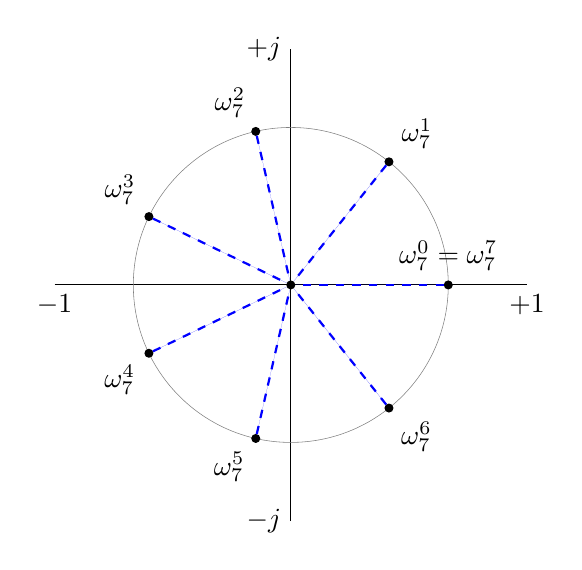
\begin{tikzpicture}[
  dot/.style={draw,fill,circle,inner sep=1pt}
  ]
  \draw[-] (-3,0) -- (3,0) node[below] {$+1$};
  \node[below] at (-3,0) {$-1$};
  \draw[-] (0,-3) -- (0,3) node[left] {$+j$};
  \node[left] at (0,-3) {$-j$};
  \draw[help lines] (0,0) circle (2);

  \node[dot] (zero) at (0,0) {};
  % default line width=0.4pt
  \foreach \i in {1,...,\nminusone} {
    \node[dot,label={\i*360/\n-(\i==\n)*45:$\omega_{\n}^{\i}$}] (w\i) at (\i*360/\n:2) {};
    %\draw[->,dashed] (O) -- (w\i);
    \path[draw=blue,fill=blue,dashed,line width=0.8pt] (w\i) -- (zero);
  }
  % draw 0 and n
  \node[dot,label={90:$\omega_{\n}^{0} = \omega_{\n}^{\n}$}] (w0) at (0:2) {};
  %\draw[->,dashed] (zero) -- (w0);
  \path[draw=blue,fill=blue,dashed,line width=0.8pt] (w0) -- (zero);
\end{tikzpicture}
}

  \captionof{figure}[The 7th complex roots of unity in the complex plane.]{
    The values of the $7$th complex roots $\omega_7^0, \dotsc, \omega_7^6$ in
    the complex plane, where $\omega_7^7 = e^{2 \pi \frac{j}{7}}$ is the
    principal $7$th root of unity.\label{fig:roots7}
  }
\end{center}

The $n$ complex $n$th roots of unity $\omega_n^0, \dotsc, \omega_n^{n - 1}$
form a group under multiplication with the same structure as the additive
group $(\bbZ_n, +)$ modulo $n$, since $\omega_n^n = \omega_n^0 = 1$ implies
that $\omega_n^k \omega_n^i = \omega_n^{k + i} = \omega_n^{(k + i)
  \bmod{n}}$. Similarly, $\omega_n^{-1} = \omega_n^{n - 1}$.

We now present some lemmas to better understand some essential properties of
complex $n$th roots of unity. We refer to \cite{Cormen:2009:IAT:1614191} for
the full proofs.

\begin{lemma}[Cancelation lemma {\autocite[Lemma~30.3]{Cormen:2009:IAT:1614191}}]
  For any integers $n \geq 0$, $k \geq 0$, and $d > 0$,
  \begin{equation}
    \omega_{d n}^{d k} = \omega_n^k
    \label{eq:complex-cancel}
  \end{equation}
  \label{lemma:complex-cancel}
\end{lemma}

\begin{corollary}[{\autocite[Corollary~30.4]{Cormen:2009:IAT:1614191}}]
  For any integer $n > 0$,
  \begin{equation}
    \omega_n^{n/2} = \omega_2 = -1
    \label{eq:waeva}
  \end{equation}
  \label{coro:waeva}
\end{corollary}

\begin{lemma}[Halving lemma {\autocite[Lemma~30.5]{Cormen:2009:IAT:1614191}}]
  If $n > 0$ is even, then the squares of the $n$ complex $n$th roots of unity
  are the $n / 2$ complex $(n / 2)$th roots of unity.
  \label{lemma:halving}
\end{lemma}

\begin{lemma}[Summation lemma {\autocite[Lemma~30.6]{Cormen:2009:IAT:1614191}}]
  For any integer $n \geq 1$ and non-zero integer $k$ not divisible by $n$,
  \begin{equation}
    \sum_{i = 0}^{n - 1}{\left( \omega_n^k \right)^i} = 0
    \label{eq:summation}
  \end{equation}
  \label{lemma:summation}
\end{lemma}

\subsection{Discrete Fourier Transform}
We want to evaluate a polynomial $A(x)$ of degree-bound $n$ at the $n$ complex
$n$th roots of unity\footnotemark.
%We wish to evaluate a polynomial $A(x)$ of degree-bound $n$ at $n$ point-value
%pairs\footnotemark.
%More precisely, at the $n$ complex $n$th roots of unity $\omega^0_n, \dotsc,
%\omega^{n - 1}_n$.
Assuming that $A(x)$ is given in coefficient form $a = (\setSpace{a}{0}{n-1})$,
we want to obtain a vector $y = (\setSpace{y}{0}{n-1})$, where each $y_k$ is of
the form:
\begin{align}
  y_k\ &=\  A(\omega_n^k) \nonumber \\
       &=\  \sum_{i = 0}^{n - 1}{a_i \omega_n^{k i}}
  \label{eq:dft}
\end{align}
\footnotetext{In the context of polynomial multiplication, the length $n$ is
actually $2n$, but for clarity we use $n$ instead of $2n$ in this section.}

The vector $y$ is the \emph{Discrete Fourier Transform} of the coefficient
vector $a$, or more succinctly, $y = \DFT_n(a)$. Note that this still takes
$\Theta(n^2)$ time.

\subsection{Fast Fourier Transform}
By using a \emph{fast Fourier Transform}, which takes advantage of the special
properties of the complex roots of unity, it is possible to compute $\DFT_n(a)$
in time $\Theta(n \log{n})$. It is assumed that $n$ is a power of $2$.

The FFT technique uses a divide-and-conquer strategy by dividing $A(x)$ into
two polynomials of degree-bound $n/2$:
%The FFT technique uses a divide-and-conquer strategy, using the even-indexed
%and the odd-indexed coefficients of $A(x)$ separately to define the two new
%polynomials $A^{(0)}(x)$ and $A^{(1)}(x)$ of degree-bound $n/2$:
\begin{align*}
  A^{(0)}(x) = a_0 + a_2 x + a_4 x^2 + \dotsc + a_{n - 2} x^{n/2 - 1} \\
  A^{(1)}(x) = a_1 + a_3 x + a_5 x^2 + \dotsc + a_{n - 1} x^{n/2 - 1}
\end{align*}
Because $A^{(0)}$ contains all the even-indexed coefficients and $A^{(1)}$
contains all the odd-indexed coefficients, we have that:
%Because $A^{(0)}$ contains all the even-indexed coefficients (the binary
%representation of the index ends in 0) and $A^{(1)}$ contains all the
%odd-indexed coefficients (the binary representations of the index ends in 1),
%it follows that:
\begin{equation}
  A(x) = A^{(0)}(x^2) + x A^{(1)}(x^2).
  \label{eq:poly-fft1}
\end{equation}

So basically, the problem of evaluating $A(x)$ at the $n$ complex $n$th roots
of unity reduces to:
\begin{enumerate}
  \item \label{enum:eval1} evaluate the degree-bound $n/2$ polynomials
    $A^{(0)}(x)$ and $A^{(1)}(x)$ at the points $(\omega_n^0)^2, \dotsc,
    (\omega_n^{n - 1})^2$, and then
  \item \label{enum:eval2} combine the results according to
    \refequation{eq:poly-fft1}.
\end{enumerate}

Because of \reflemma{lemma:halving} (halving lemma), the list of points in
(\ref{enum:eval1}) has not $n$ distinct values but only $n/2$ complex $(n/2)$th
roots of unity, with each root occurring exactly twice.  This means that we can
divide a $n$-element $\DFT_n$ computation into two $n/2$-element $\DFT_{n/2}$
computations. This is the basis for the definition of the recursive FFT
algorithm, which computes the DFT of an $n$-element vector $a
= (\setSpace{a}{0}{n-1})$, with $n$ a power of $2$. Such algorithm is presented
in \refalg{alg:rec-fft}.
%Because of \reflemma{lemma:halving} (halving lemma), the list of points in
%(\ref{enum:eval1}) has not $n$ distinct values but only $n/2$ complex $(n/2)$th
%roots of unity, with each root occurring exactly twice. So we recursively
%evaluate the polynomials $A^{(0)}$ and $A^{(1)}$ of degree-bound $n/2$ at the
%$n/2$ complex $(n/2)$th roots of unity. These sub-problems are exactly like the
%original problem, but are half the size. In short, we can divide a $n$-element
%$\DFT_n$ computation into two $n/2$-element $\DFT_{n/2}$ computations. With
%this decomposition we can now define the recursive FFT algorithm, which
%computes the DFT of an $n$-element vector $a = (a_0, \dotsc, a_{n - 1})$, with
%$n$ a power of $2$.

\begin{algorithm}
  \begin{algorithmic}[1]
    \Function{Recursive-FFT}{a}
      \State $n \gets a.length$
      \If{n == 1}
        \State \Return a
      \EndIf
      \State $\omega_n \gets e^{2 \pi \rfrac{j}{n}}$
      \State $\omega \gets 1$
      \State $a^{(0)} \gets (a_0, a_2, \dotsc, a_{n - 2})$
      \State $a^{(1)} \gets (a_1, a_3, \dotsc, a_{n - 1})$
      \State $y^{(0)} \gets $\Call{Recursive-FFT}{$a^{(0)}$}
      \State $y^{(1)} \gets $\Call{Recursive-FFT}{$a^{(1)}$}
      \For{$k = 0$ \textbf{to} $n/2 - 1$}
        \State $y_k \gets y_k^{(0)} + \omega\ y_k^{(1)}$
        \State $y_{k + (n/2)} \gets y_k^{(0)} - \omega\ y_k^{(1)}$
        \State $\omega \gets \omega\ \omega_n$
      \EndFor
      \State \Return $y$
    \EndFunction
  \end{algorithmic}
  \caption{Recursive FFT.}
  \label{alg:rec-fft}
\end{algorithm}


%Looking at \textsc{Recursive-FFT}, the lines 3--5 represent the basis of
%recursion; the DFT of a vector with one element is the element itself:
%\begin{align*}
%  y_0 &= a_0 \omega_1^0 \tag*{(by \refequation{eq:dft})} \\
%    &= a_0 \cdot 1 \\
%    &= a_0
%\end{align*}
%
%On lines 8--9 the input coefficient list is split into two. Lines 6, 7 and 15
%guarantee that the $\omega$ value is updated correctly so that when lines
%13--14 are executed we always have $\omega = \omega_n^k$. Lines 10--11 perform
%the recursive $\DFT_{n/2}$ computations, setting, for $0 \leq k < \frac{n}{2}$:
%\begin{align*}
%  y_k^{(0)} &= A^{(0)}(\omega_{n / 2}^k) &
%  y_k^{(1)} &= A^{(1)}(\omega_{n / 2}^k) \\
%  %
%  &= A^{(0)}(\omega_n^{2 k}) &
%  &= A^{(1)}(\omega_n^{2 k}) \tag*{(by \reflemma{lemma:complex-cancel})}
%\end{align*}
%
%Lines 13--14 combine the results of the recursive $\DFT_{n/2}$ calculations.
%For $0 \leq k < \frac{n}{2}$, line 13 gives:
%\begin{align*}
%  y_k &= y_k^{(0)} + \omega_n^k y_k^{(1)} \\
%      &= A^{(0)}(\omega_n^{2 k}) + \omega_n^k A^{(1)}(\omega_n^{2 k}) \\
%      &= A(\omega_n^k) \tag*{(by \refequation{eq:poly-fft1})}
%\end{align*}
%In line 14, for $0 \leq k < \frac{n}{2}$, we have:
%\begin{align*}
%  y_{k + (n / 2)} &= y_k^{(0)} - \omega y_k^{(1)} \\
%                  &= y_k^{(0)} + \omega_n^{k+(n/2)} y_k^{(1)} \tag*{(since
%                    $\omega_n^{k+(n/2)} = - \omega_n^k$)} \\
%                  &= A^{(0)}(\omega_n^{2k}) + \omega_n^{k+(n/2)}
%                    A^{(1)}(\omega_n^{2k}) \tag*{(by
%                    \reflemma{lemma:complex-cancel})}\\
%                  &= A^{(0)}(\omega_n^{2k + n}) + \omega_n^{k+(n/2)}
%                    A^{(1)}(\omega_n^{2k + n}) \tag*{(since $\omega_n^{2k+n}
%                    = \omega_n^{2k}$)}\\
%                  &= A(\omega_n^{k + (n / 2)}) \tag*{(by
%                    \refequation{eq:poly-fft1})}
%\end{align*}
%So the $y$ vector returned by \textsc{Recursive-FFT} is indeed the $\DFT$ of
%the input vector a.

To analyze the running time of \refalg{alg:rec-fft}, note that each invocation
of the function \textsc{Recursive-FFT} (excluding the recursive calls) takes
$\Theta(n)$ time, where $n$ is the length of the input vector. Therefore, the
recurrence for the running time is:
\begin{align*}
  T(n) \quad &= \quad 2T(n / 2) + \Theta(n) \\
             &= \quad \Theta(n \log{n})
\end{align*}

In other words, we can perform the evaluation of a polynomial of degree-bound
$n$ at the complex $n$th roots of unity in time $\Theta(n \log{n})$ using the
FFT.

\subsection{Interpolation at the complex roots of unity}
To complete the polynomial multiplication method we just need to interpolate
the complex roots of unity by a polynomial, so that after we can convert the
point-value representation back to coefficient representation.
%Essentially, we write the DFT as a matrix equation and then look at the form of
%the matrix inverse.

\begin{comment}
First, we can write the equation $y_k = A(x_k)$ for $k = 0, \dotsc, n - 1$ as
a matrix equation:
\begin{equation}
  \begin{pmatrix*}
    1      & x_0     & x_0^2       & \cdots  & x_0^{n - 1}     \\
    1      & x_1     & x_1^2       & \cdots  & x_1^{n - 1}     \\
    \vdots & \vdots  & \vdots      & \ddots  & \vdots          \\
    1      & x_{n-1} & x_{n-1}^2   & \cdots  & x_{n-1}^{n - 1}
  \end{pmatrix*}
  \begin{pmatrix*}
    a_0     \\
    a_1     \\
    \vdots  \\
    a_{n-1} 
  \end{pmatrix*}
  =
  \begin{pmatrix*}
    y_0       \\
    y_1       \\
    \vdots    \\
    y_{n - 1}
  \end{pmatrix*}
  \label{eq:uniq-poly-inter}
\end{equation}

The matrix in the left, denoted as $V(\setSpace{x}{0}{n-1})$, is known as the
Vandermonde matrix. This square matrix has determinant of:
\begin{equation*}
  \prod_{0 \leq i < k < n}{(x_k - x_i)}
\end{equation*}
and therefore, the Vandermonde matrix is known to be invertible if and only if
the $x_k$ are distinct. So the previous matrix equation can be written as: $a
= V(\setSpace{x}{0}{n-1})^{-1} y$.

From \refequation{eq:uniq-poly-inter}, we can write the DFT as the matrix
product (we are multiplying the Vandermonde matrix $V_n$ containing the
appropriate powers of $\omega_n$ by $a$):
\begin{equation*}
  \begin{pmatrix*}
    y_0     \\
    y_1     \\
    y_2     \\
    \vdots  \\
    y_{n - 1}
  \end{pmatrix*}
  =
  \begin{pmatrix*}
    1     &    1          &    1            &\cdots&      1                 \\
    1     &\omega_n       &\omega_n^2       &\cdots&\omega_n^{n - 1}        \\
    1     &\omega_n^2     &\omega_n^4       &\cdots&\omega_n^{2(n - 1)}     \\
    \vdots&\vdots         &\vdots           &\ddots&\vdots                  \\
    1     &\omega_n^{n-1} &\omega_n^{2(n-1)}&\cdots&\omega_n^{(n-1)(n - 1)}
  \end{pmatrix*}
  \begin{pmatrix*}
    a_0     \\
    a_1     \\
    a_2     \\
    \vdots  \\
    a_{n-1}
  \end{pmatrix*}
\end{equation*}
Each $(i,k)$ entry of $V_n$ is $\omega_n^{i k}$ for $i, k = 0, \dotsc, n - 1$.

For the inverse operation, written as $a = \DFT_n^{-1}(y)$, and since we
known that $V_n$ is invertible, we proceed by multiplying $y$ by $V_n^{-1}$.

\begin{theorem}[{\autocite[Theorem~30.7]{Cormen:2009:IAT:1614191}}]
  For $i, k = 0, \dotsc, n - 1$, the $(i,k)$ entry of $V_n^{-1}$ is
  $\omega_n^{-k i}/n$.
  \label{theo:vande}
\end{theorem}
\end{comment}

Essentially, we want to compute the inverse DFT, denoted as  $\DFT_n^{-1}(y)$.
The inverse DFT is given by:
\begin{equation}
  a_i = \frac{1}{n} \sum_{k = 0}^{n - 1}{y_k \omega_n^{-k i}} \qquad 0 \leq
  i < n
  \label{eq:dft-inv}
\end{equation}

If we compare the DFT of \refequation{eq:dft} with \refequation{eq:dft-inv}, we
see that we can use the FFT (\refalg{alg:rec-fft}) to compute both the DFT and
its inverse as well. We simply switch the roles of $a$ and $y$, replace
$\omega_n$ by $\omega_n^{-1}$, and divide each element of the result by $n$.
Thus, we can compute the $\DFT_n^{-1}$ in $\Theta(n \log{n})$ time as well.

Having the DFT and its inverse, we can use FFT to transform a polynomial of
degree-bound $n$ back and forth between its coefficient and point-value
representation in time $\Theta(n \log{n})$.

For the polynomial multiplication, we have the \emph{convolution} theorem
defined as follows:
\begin{theorem}[{\autocite[Theorem~30.8]{Cormen:2009:IAT:1614191}}]
  For any two vectors $a$ and $b$ of length $n$, where $n$ is a power of 2,
  \begin{equation*}
    a \otimes b = \DFT_{2n}^{-1}(\DFT_{2n}(a) \cdot \DFT_{2n}(b))
  \end{equation*}
  where the vectors $a$ and $b$ are padded with $0$s in order to have length
  $2n$ and the operator $\cdot$ denotes the component-wise product of two
  $2n$-element vectors.
  \label{eq:convolution}
\end{theorem}

This basically concludes the polynomial multiplication algorithm based on FFT,
with $\Theta(n \log{n})$ time.
